\section*{Physique (13 points)}
\section{Propagation d'une onde à la surface de l'eau}
La cuve à ondes peut être utilisée comme dispositif pour étudier la propagation
des ondes. Selon les conditions de l'expérience, on peut assister aux phénomènes
de propagation et de diffraction ce qui permet d'identifier certaines
caractéristiques des ondes et du milieu de propagation.

À l'aide du vibreur de la cuve à ondes, on crée à $t_{0}=0$ en un point $S$ de
la surface libre de l'eau une onde progressive sinusoïdale de fréquence
$\freq=\qty{20}{\Hz}$.

\begin{enumerate}
    \item L'onde se propage à la surface de l'eau avec une célérité $v$ sans
          amortissement ni réflexion.
          \begin{enumerate}
              \item Définir une onde mécanique progressive sinusoïdale.
              \item L'onde étudiée est-elle longitudinale ou transversale~?
                    Justifier.
          \end{enumerate}
    \item \mbox{}
          \begin{minipage}[t][][t]{0.76\linewidth}
              La figure ci-contre schématise l'aspect de la surface de l'eau à
              un instant $t$ où les cercles représentent les crêtes.

              Recopier, sur votre copie, le numéro de la question et choisir la
              lettre correspondante à la proposition vraie.
          \end{minipage}
          \hfill
          \begin{minipage}[t][][t]{0.20\linewidth}
              \begin{figure}[H]
                  \centering
                  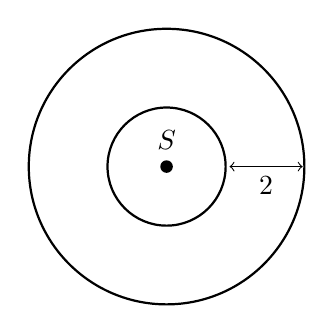
\begin{tikzpicture}[]
                      \node[circle,fill,inner sep=1.6pt,label=$S$] (S) {};
                      \node[circle,draw,thick,inner sep=0pt,
                            minimum size=1.5cm] (C1) {};
                      \node[circle,draw,thick,inner sep=0pt,
                            minimum size=3.5cm] (C2) {};
                      \draw[<->,shorten <=1pt,shorten >=1pt] (C1.east) -- 
                          node[below] {$\qty{2}{\cm}$} (C2.east);
                  \end{tikzpicture}
              \end{figure}
          \end{minipage}

          \vspace{-2cm}
          \begin{enumerate}
              \item La valeur de la longueur d'onde $\lambda$ est~:
          
                    \begin{enumerate*}[label=\fbox{\Alph{enumiii}},
                            itemjoin=\hspace{1cm}]
                        \item $\lambda=\qty{1}{\cm}$
                        \item $\lambda=\qty{1.5}{\cm}$
                        \item $\lambda=\qty{2}{\cm}$
                        \item $\lambda=\qty{2.5}{\cm}$
                    \end{enumerate*}
              \item La valeur de la vitesse de propagation de l'onde à la
                    surface de l'eau est~: \par
                    \begin{enumerate*}[label=\fbox{\Alph{enumiii}},itemjoin=\hfill]
                        \item $v=\qty{0.4}{\m\per\s}$
                        \item $v=\qty{0.3}{\m\per\s}$
                        \item $v=\qty{0.2}{\m\per\s}$
                        \item $v=\qty{0.15}{\m\per\s}$
                    \end{enumerate*}
          
              \item Les points situés à la distance $d=\qty{4}{\cm}$ de $S$
                    sont atteints par l'onde à l'instant $t_{1}$.
          
                    La valeur de $t_{1}$ est~: \par
                    \begin{enumerate*}[label=\fbox{\Alph{enumiii}},itemjoin=\hfill]
                        \item $t_{1}=\qty{0.2}{\s}$
                        \item $t_{1}=\qty{0.15}{\s}$
                        \item $t_{1}=\qty{0.1}{\s}$
                        \item $t_{1}=\qty{0.05}{\s}$
                    \end{enumerate*}
          \end{enumerate}


    \item On considère le point $M$ de la surface de l'eau situé au repos à la
          distance $d=\qty{4}{\cm}$ de la source $S$. Écrire l'élongation
          $y_{M}(t)$ du point $M$ en fonction de l'élongation de la source $S$.
  
    \item On règle la fréquence du vibreur sur la valeur
          $\freq^{\prime}=\qty{10}{\Hz}$, on obtient à la surface de l'eau une onde
          de longueur d'onde $\lambda^{\prime}=\qty{3}{\cm}$. Déduire, en
          justifiant la réponse, une propriété du milieu de propagation.
    \item On excite à nouveau la surface de l'eau avec une réglette mince, on
          obtient une onde rectiligne progressive périodique de fréquence
          $\freq=\qty{20}{\Hz}$ qui se propage à la vitesse
          $v=\qty{0.4}{\m\per\s}$.

          On place un obstacle muni d'une ouverture de largeur
          $a=\qty{0.5}{\cm}$ sur le trajet des ondes.
          \begin{enumerate}
              \item Justifier que l'onde subit la diffraction après la traversée
                    de l'ouverture.
              \item Donner les caractéristiques de l'onde après la traversée de
                    l'ouverture.
          \end{enumerate}
\end{enumerate}






\section*{Excrcice 2 (5 points)~: Dipule RC - Dipdie RL - Circuit/G}
L'étude du condensateur, de la bobine ou de leur association peut se faire en se basant sur une étude expérimentale. La réponse des dipôles associés à ces composants fournit des informations sur le comportement de chacun, sur la nature des oscillations électriques dans un circuit $L C$ ainsi que sur les aspects et échanges énergétiques à leurs niveaux.\\
Cet exercice vise~:

\begin{itemize}
  \item la détermination de la capacité d'un condensateur~;
  \item la détermination de l'inductance d'une bobine~;
  \item l'étude des oscillations électriques libres dans un circuit LC.
\end{itemize}

\section*{Partie 1~: Détermination de la capacité d'un condensateur}
On considère le circuit représenté sur la figure l où le générateur débite dans le circuit un courant électrique d'intensité constante $I_{0}=14,1 \mathrm{~mL}$.

\begin{figure}[h]
\begin{center}
  \includegraphics[width=\textwidth]{c8da97a1-45e2-47e7-8c6c-2b3cd6681557-4}
\captionsetup{labelformat=empty}
\caption{Figure 1}
\end{center}
\end{figure}

On ferme l'interrupteur à l'instant $t_{0}=0$. L'étude des variations de la tension $u_{C}$ aux bornes du condensateur de capacité $C$ permet de tracer la courbe de la figure 2.

\begin{enumerate}
  \item Préciser parmi les armatures A et B du condensateur, celle portant les charges positives.
  \item Dans l'intervalle $0 \leq t \leq 3 \mathrm{~ms}$, établir l'expression $u_{C}=\frac{I_{0}}{C} t$.
  \item Vérifier que $C=14,1 \mu F$.
  \item Calculer la valeur maximale $\mathcal{E}_{e, \text { max }}$ de l'énergie électrique emmagasinée dans le condensateur.
\end{enumerate}

\begin{figure}[h]
\begin{center}
  \includegraphics[width=\textwidth]{c8da97a1-45e2-47e7-8c6c-2b3cd6681557-4(1)}
\captionsetup{labelformat=empty}
\caption{Figure 2}
\end{center}
\end{figure}

\section*{Partie 2~: Détermination de Pinductance d'unc bobine}
On considère le circuit de la figure 3, qui comporte~:

\begin{itemize}
  \item un générateur idéal de tension de fé.m $E=6 V$~;
  \item un conducteur olmique de résistance $R=30 \Omega$~;
  \item une bobine d'inductance $L$ et de résistance négligeable~:
  \item un interrupteur $K$.
\end{itemize}

A l'instant $t_{0}=0$, on ferme $K$. La figure 4 représente la courbe de la

\begin{figure}[h]
\begin{center}
  \includegraphics[width=\textwidth]{c8da97a1-45e2-47e7-8c6c-2b3cd6681557-5(1)}
\captionsetup{labelformat=empty}
\caption{Figure 3}
\end{center}
\end{figure}

tension $u_{R}(t)$ entre les bomes du conducteur ohmique.

\begin{enumerate}
  \item Montrer que l'équation différentielle vérifiée par la tension $u_{A}$ s'écrit $\frac{L}{R} \cdot \frac{d u_{n}}{d t}+u_{n}=E$.
  \item La solution de cette équation diffèrentielle s'écrit $u_{n}(t)=A\left(1-e^{-t *}\right)$ où $A$ et $\tau$ sont des constantes.\\
2.1. Exprimer $A$ et r en fonction des paramètres du circuit.\\
2.2. Vérifier que $L=0,18 H$.
\end{enumerate}

\begin{figure}[h]
\begin{center}
  \includegraphics[width=\textwidth]{c8da97a1-45e2-47e7-8c6c-2b3cd6681557-5(2)}
\captionsetup{labelformat=empty}
\caption{Figure 4}
\end{center}
\end{figure}

\section*{Partic 3~: Étude des oscillations électriques libres dans un circuit L.C}
On monte le condensateur préeèdent de capacité $C$ en série avec la bobine précédente.\\
Le condensateur étant totalement chargé à $t_{0}=0$.\\
La courbe de la figure 5 représente la tension $u_{c}(t)$ entre les bornes du condensateur.

\begin{enumerate}
  \item Nommer le régime d'oscillations électriques dans le circuit.
  \item Déterminer graphiquement la valeur de la période propre $T_{0}$ de l'oscillateur (LC).
  \item Déterminer la valeur de l'énergie totale 8 du circuit.
  \item Indiquer, sous quelle forme. l'énergie se repartit dans le
\end{enumerate}

\begin{figure}[h]
\begin{center}
  \includegraphics[width=\textwidth]{c8da97a1-45e2-47e7-8c6c-2b3cd6681557-5}
\captionsetup{labelformat=empty}
\caption{Figure 5}
\end{center}
\end{figure}

\section*{Excrcice 3 (3.5 wints)~: Chutelibre-Systemc oscillant (Sollde-Ressort)}
Les mouvements des corps sont dus à des actions mécaniques. Les forces associées
à ces actions peuvent être constantes ou variables. L'application de telles
forces engendre des mouvements différents et permet de déterminer certaines
caractéristiques de ces mouvements.

Cet exercice vise~:
\begin{itemize}
    \item l'étude du mouvement d'un solide soumis à une force constante~;
    \item l'étude du mouvement d'un solide soumis à une force variable.
\end{itemize}

\subsection{Étude du mouvement d'une bille en chute libre}
\begin{minipage}[t][][t]{0.78\linewidth}
    À un instant choisi comme origine de temps ($t_{0}=0$), on lance verticalement
    vers le haut avec une vitesse initiale $\vec{V}_{0}$ une bille de masse $m$
    d'une position $A$ située à la hauteur $h=\qty{1.2}{\m}$ du sol.
    
    On étudie le mouvement du centre d'inertie $G$ de la bille dans un référentiel
    terrestre considéré galiléen. On repère la position de $G$ à un instant $t$ par
    son abscisse $z_{G}$ dans le repère ($O,\vec{k}$) où $z_{A}=0$
    (Fig.~\ref{fig:2bac_svt_national_2024_normale_phys_ex3_1}).
    
    \begin{enumerate}
        \item En appliquant la deuxième loi de \textsc{Newton}, établir l'équation
              différentielle vérifiée par l'abscisse $z_{G}$.
        \item Déterminer la nature du mouvement de $G$.
        \item L'équation de la vitesse de $G$ durant son mouvement s'écrit\\
              ${v_{G}=10\cdot t-4 \quad (\unit{\m\per\s})}$.
              \begin{enumerate}
                  \item Déterminer la valeur de l'instant $t_{1}$ où $G$ atteint la
                        hauteur maximale.
                  \item Déterminer la valeur de la hauteur maximale $h_{m}$ atteinte
                        par $G$ par rapport au sol.
              \end{enumerate}
    \end{enumerate}
\end{minipage}
\hfill
\begin{minipage}[t][][t]{0.2\linewidth}
\begin{figure}[H]
	\centering
    \begin{tikzpicture}[thick]
        \def\h{4}
        \def\xA{1}
        \coordinate (O) at (0,0);
        \draw[-Latex] (0,2) -- (0,-\h) node[left,pos=0.98] {$z$};
        \draw[very thick] (3pt,0) -- (-3pt,0) node[left] {$O$};
        \draw[->,very thick] (O) -- ++(0,-1) node[left,pos=0.8] {$\vec{k}$};
        \node[circle,fill=gray,draw,inner sep=5pt,
              label=above left:$A$] (S) at (\xA,0) {};
        \draw[->] (S.center) -- ++(0,1) node[right,pos=0.85] {$\vec{V}_{0}$};
        \draw[densely dashed,thin] (O) -- +(2.5*\xA,0);
        \node[minimum width=3cm,minimum height=3mm,top color=black!80,
              anchor=north west] at (-.5,-\h) {};
        \draw[<->,shorten <=1pt,shorten >=1pt]
            (2*\xA,0) -- node[right] {$h$} +(0,-\h);
    \end{tikzpicture}
	\caption{}
	\label{fig:2bac_svt_national_2024_normale_phys_ex3_1}
\end{figure}
\end{minipage}


\subsection{Étude du mouvement de l'oscillateur (Solide - Ressort)}
On considère un système oscillant (solide-ressort horizontal) où la valeur de la
masse du solide est $m=\qty{125}{\gram}$ et la raideur du ressort est noté $K$.

\begin{minipage}{0.65\linewidth}
    L'équation horaire du mouvement du centre d'inertie $G$ du solide s'écrit
    $x=X_m \cos \left(\frac{2\pi}{T_0} t\right)$.

    La courbe de la Fig.~\ref{fig:2bac_svt_national_2024_normale_phys_ex3_2}
    représente l'élongation $x$ du mouvement de $G$.

    \begin{enumerate}
        \item Déterminer graphiquement les valeurs des grandeurs $X_m$ et
              $T_0$.
        \item Vérifier que $K=\qty{19.7}{\newton\per\meter}$
        \item Déterminer l'intensité de la force de rappel exercée par le
              ressort sur le solide a l'instant $t=\frac{5}{2} T_0$.
    \end{enumerate}
\end{minipage}
\hfill
\begin{minipage}{0.34\linewidth}
\begin{figure}[H]
    \centering
    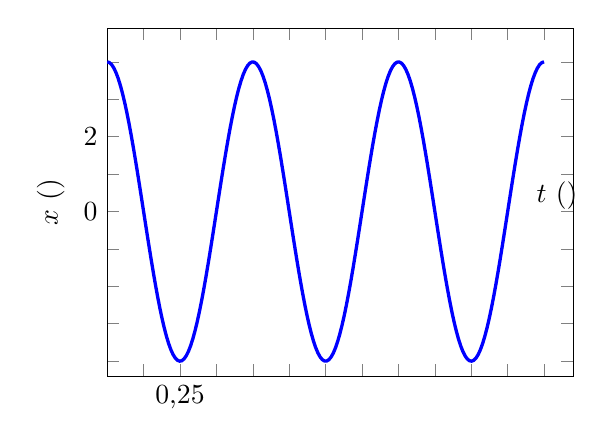
\begin{tikzpicture}
        \def\Xm{4}
        \def\T{0.5}
        \pgfmathpi\let\pi=\pgfmathresult
        \begin{axis}[
                xmin=0,xmax=3.2*\T,
                ymin=-4.4,ymax=4.9,
                width=7.5cm,height=6cm,
                trig format plots=rad,
                xtick distance=0.125, ytick distance=1,
                xticklabels={,,,{0,25}}, yticklabels={,,,,,0,,2},
                xlabel=$t~(\unit{\second})$, ylabel=$x~(\unit{\cm})$,
                every axis x label/.append style={
                	at={(1.03,0.45)},anchor=south east,
                },
                minor tick num=0,
            ]
            \addplot[domain=0:3*\T,samples=200,very thick,blue]
                {\Xm*cos(2*pi/\T*x)};
        \end{axis}
    \end{tikzpicture}
    \caption{}
    \label{fig:2bac_svt_national_2024_normale_phys_ex3_2}
\end{figure}
\end{minipage}





